% Supplementary material for the Bioinformatics Application Note
%   "qPCRtools: a cross-platform C++ desktop application for qPCR data
%    analysis with validated equivalence to its R implementation"
%
% 单独编译（与 main.tex 同级，图形路径相同）：
%   TECTONIC_CACHE_DIR="$HOME/Library/Caches/TectonicProject.Tectonic" tectonic supplementary.tex
%
% 组成（Application Note 主文只保留 1 图 1 表，其余在此）：
%   Figure S1  标准曲线 + ΔΔCt 表达量（真实数据，由仓库内脚本从同一批数值输出绘制）
%   Figure S2  C++ 与 R 的数值等价性散点（y = x）
%   Table S1   各共有方法的等价性汇总

\documentclass[11pt]{article}

\usepackage[utf8]{inputenc}
\usepackage{graphicx}
\usepackage[hidelinks]{hyperref}
\usepackage{booktabs}
\usepackage{amsmath}
\usepackage{geometry}
\geometry{margin=2.5cm}

\title{Supplementary material\\[4pt]
\large qPCRtools: a cross-platform C++ desktop application for qPCR data
analysis with validated equivalence to its R implementation}
\author{%
\parbox{\textwidth}{\centering\sloppy
Xiang Li\textsuperscript{1,2,*} \quad Huichuan Huang\textsuperscript{1,2,*}\\[6pt]
\textsuperscript{1}~State Key Laboratory for Conservation and Utilization of Bio-Resources in Yunnan,
Yunnan Agricultural University, Kunming, China\\
\textsuperscript{2}~Key Laboratory for Agro-Biodiversity and Pest Control of Ministry of Education,
Yunnan Agricultural University, Kunming, China%
}%
}
\date{}

\begin{document}
\maketitle

\section*{Contents}

\begin{itemize}
  \item Figure~S1 --- Analysis output on the bundled example data
        (standard curves and $\Delta\Delta C_t$ expression).
  \item Figure~S2 --- Numerical equivalence of the C++ implementation and the
        R package.
  \item Table~S1 --- Equivalence summary across all shared methods.
        Panel~(a): numerical equivalence with the R package.
        Panel~(b): the statistical layer (means, Welch $p$-values, ANOVA and
        Tukey letters) against an independent base-R reference.
\end{itemize}

\section{Analysis output on the bundled example data}

Figure~S1 shows the two analyses discussed in the main text, produced from the
application's numerical output by the plotting script shipped in the
repository (\texttt{code/validation/plot\_examples.py}, matplotlib), which
gives finer control over the layout than the in-interface figure export. The
per-group means, standard deviations and $p$-values were independently
reproduced without the application or the R package by
\texttt{code/validation/check\_example\_stats.R}.

\begin{figure}[h]
\centering
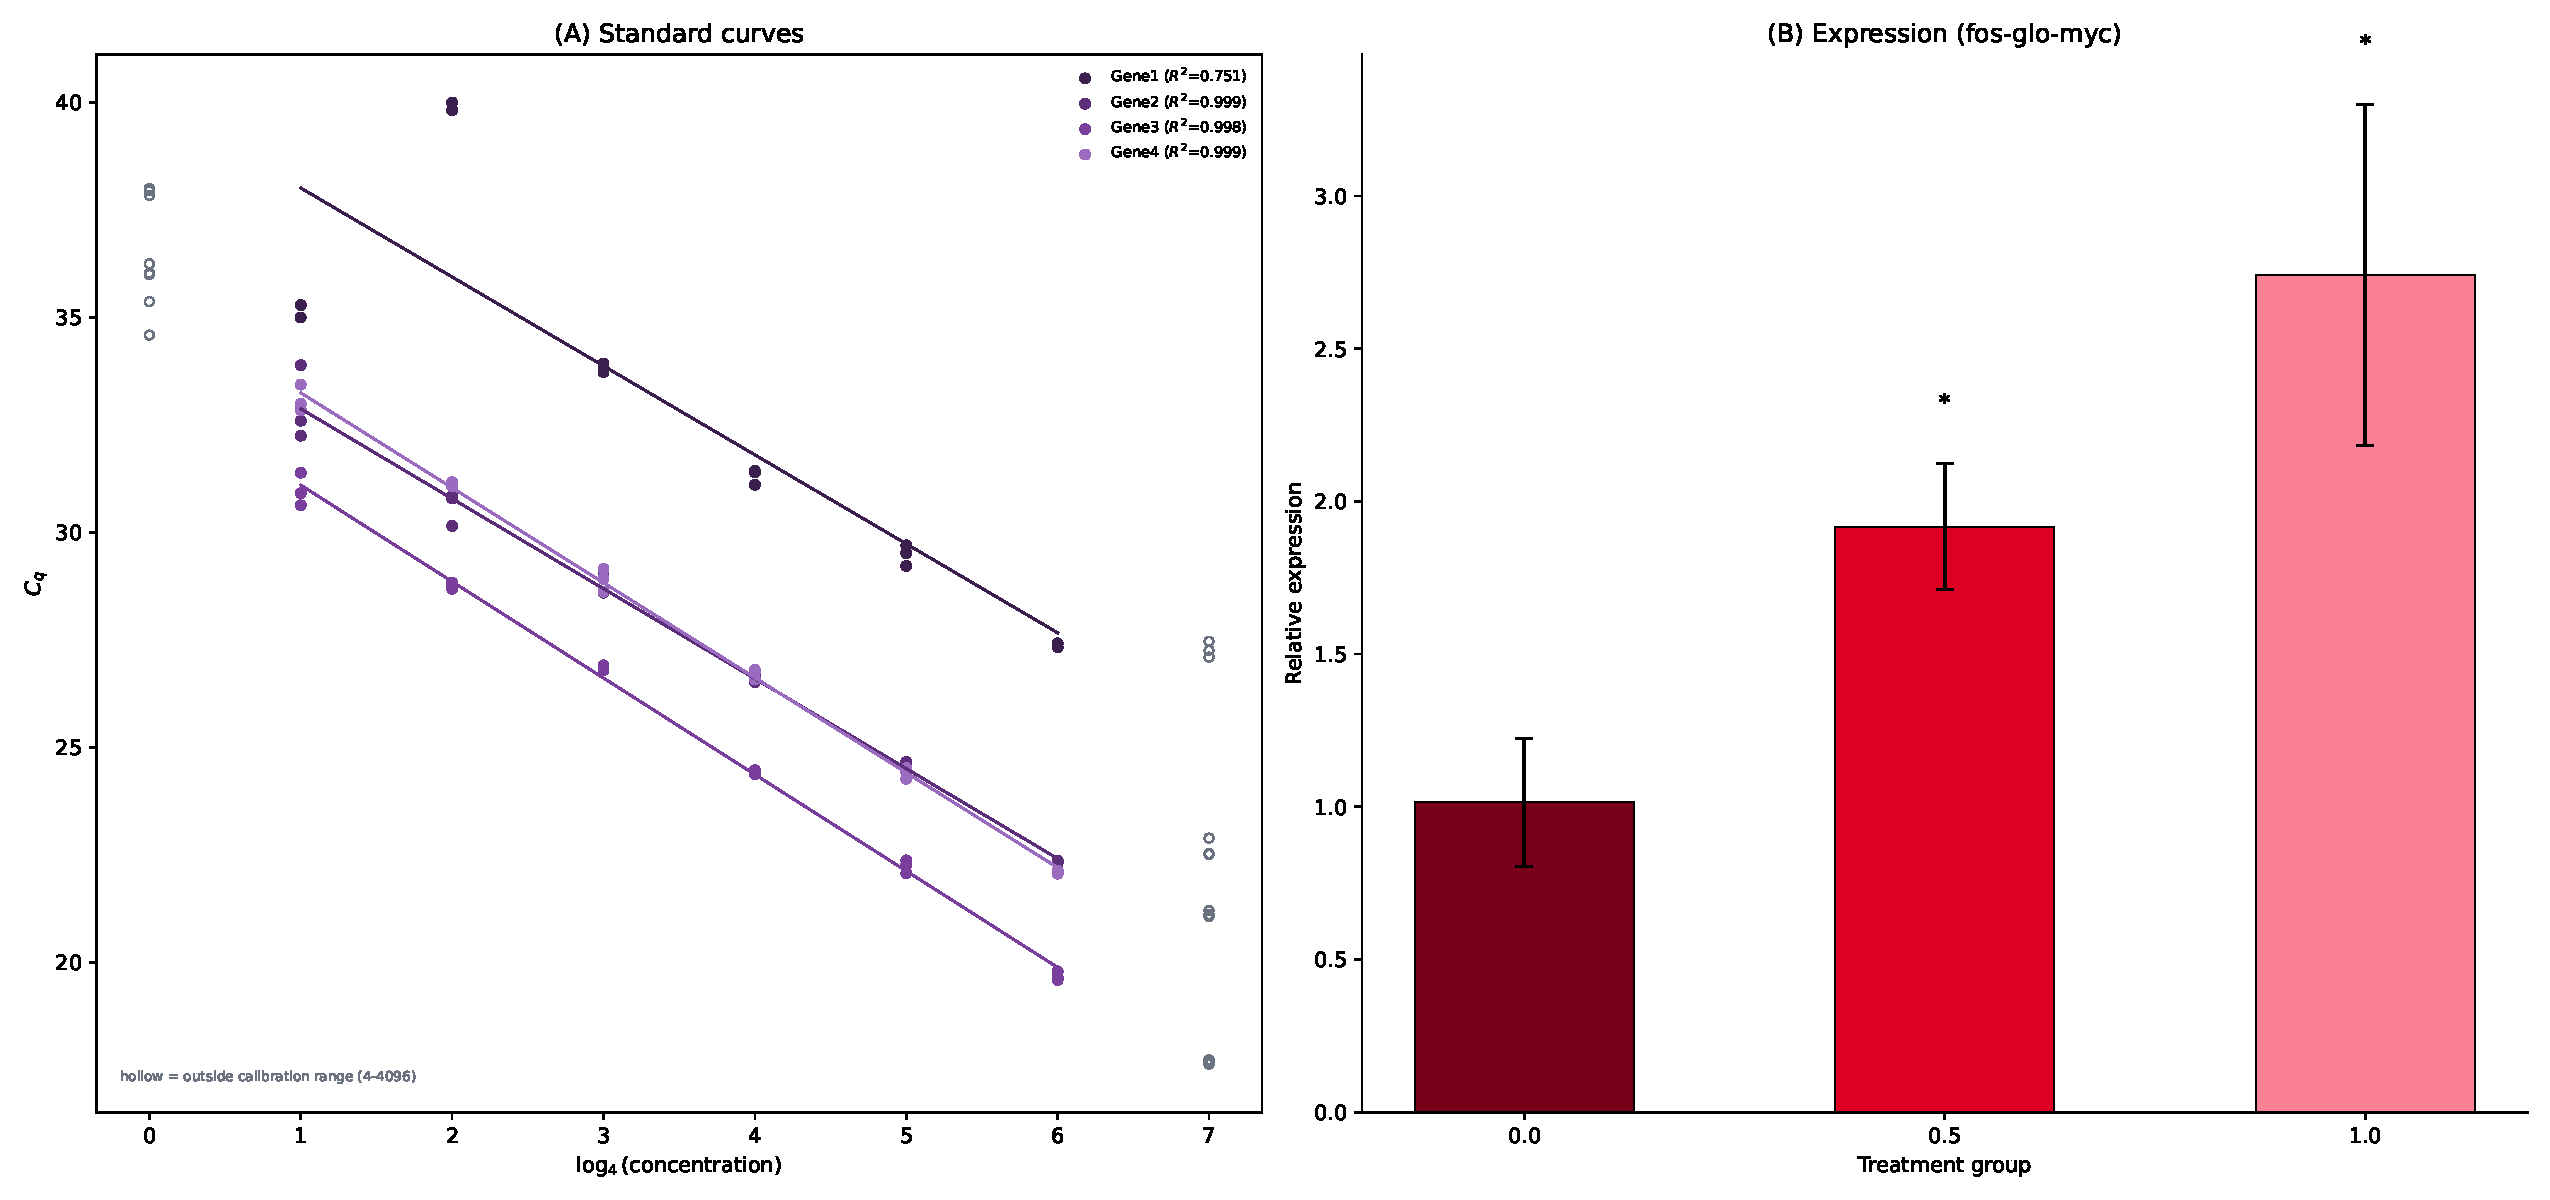
\includegraphics[width=\linewidth]{figures/fig2_results_v2.pdf}
\caption{\textbf{Figure S1.} Analysis output on real data.
(A)~Standard curves for four genes over a four-fold dilution series, with
fitted regressions and $R^2$. The abscissa is $\log_4$ concentration
(dilution steps), matching the regression, and hollow symbols mark wells
outside the calibrated range (4--4096) that are excluded from the fit.
(B)~Relative expression of \textit{fos-glo-myc} across treatment groups
($\Delta\Delta C_t$ method, calibrated to the control group), with
significance labels. Reproduced from \texttt{figures/fig2\_results\_v2.pdf}.}
\label{fig:s1}
\end{figure}

\section{Numerical equivalence to the R package}

Both implementations were run on identical input files for every shared
method---$\Delta\Delta C_t$ (\texttt{CalExp2ddCt}), the standard curve
(\texttt{CalCurve}) and the efficiency-based RqPCR method
(\texttt{CalExpRqPCR})---and every resulting quantity was compared pairwise
(Figure~S2, Table~S1).

\begin{figure}[h]
\centering
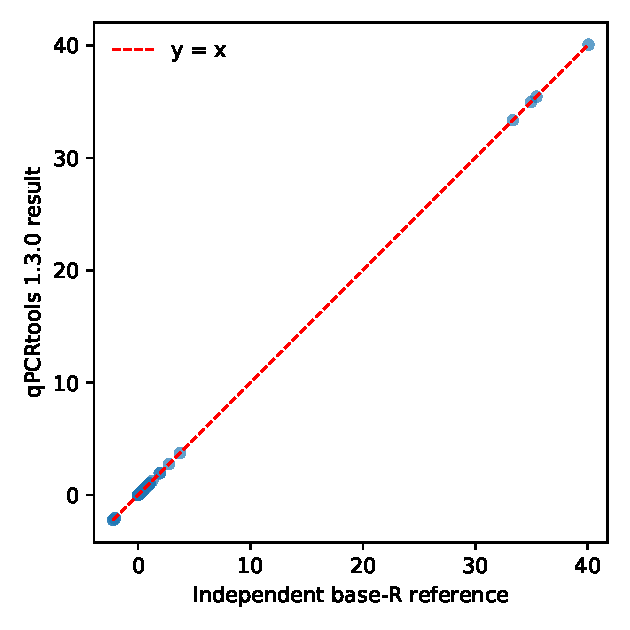
\includegraphics[width=0.62\linewidth]{figures/fig3_equivalence.pdf}
\caption{\textbf{Figure S2.} Numerical equivalence of the C++ implementation
and the R package. Each C++ result is plotted against the corresponding R
result across all shared methods; all points fall on the line $y = x$.}
\label{fig:s2}
\end{figure}

\begin{table}[h]
\centering
\caption{\textbf{Table S1.} Equivalence of the application (C++) with the
reference implementations. (a)~Numerical equivalence with the R package on
identical inputs; relative difference is $|R - \mathrm{C{+}{+}}|/|R|$.
(b)~Statistical layer on the bundled $\Delta\Delta C_t$ example, recomputed
independently in base R without installing any package
(\texttt{code/validation/verify\_stats.R}).}
\label{tab:s1}
\small
\begin{tabular}{lll}
\toprule
\multicolumn{3}{l}{\textit{(a) numerical equivalence to the R package}}\\
\midrule
Method & Compared quantities & Max.\ rel.\ diff.\ \\
\midrule
$\Delta\Delta C_t$  & expression, SD                      & $3.8 \times 10^{-15}$ \\
Standard curve      & slope, intercept, $R^2$, efficiency & $2.5 \times 10^{-3}$  \\
RqPCR               & expression, SE                      & $2.1 \times 10^{-15}$ \\
\midrule
\multicolumn{3}{l}{\textit{(b) statistical layer (bundled example, $\Delta\Delta C_t$)}}\\
\midrule
Quantity & Application (C++) & Independent base-R reference \\
\midrule
Mean $\pm$ SD, group 0.0   & $1.0145 \pm 0.2098$ & $1.0145 \pm 0.2098$ \\
Mean $\pm$ SD, group 0.5   & $1.9169 \pm 0.2060$ & $1.9169 \pm 0.2060$ \\
Mean $\pm$ SD, group 1.0   & $2.7403 \pm 0.5580$ & $2.7403 \pm 0.5580$ \\
Welch $p$ vs control       & 0.006027 / 0.022191 & 0.006027 / 0.022191 \\
ANOVA $p$ (all groups)     & 0.0034471 & 0.0034471 \\
Tukey letters              & b / ab / a & b / ab / a \\
\bottomrule
\end{tabular}
\end{table}

The residual $2.5 \times 10^{-3}$ for the standard curve is attributable to
the R package rounding its tabulated output to two to four decimal places,
since the underlying $C_q$ inputs are identical.

The statistical layer in Table~S1(b) is reproduced by an independent base-R
script that needs no package at all (\texttt{code/validation/verify\_stats.R}),
so the reported $p$-values and letter groupings can be checked without
installing the R package. The letter display is the compact letter display of
the Tukey HSD: group~0 and group~1 differ ($p_{\mathrm{adj}} = 0.0028$), whereas
group~0.5 is not separated from either ($p_{\mathrm{adj}} = 0.052$ and
$0.073$), giving b~/~ab~/~a. That borderline comparison is exactly the case in
which an incorrect multiple-comparison step is exposed, and it is covered by
both the script above and the regression tests in the repository.

\end{document}
